\subsection{Gesamtsystem}
Das Gesamtsystem wurde so günstig wie möglich aufgebaut. Wenn die einelnen Komponenten bei den preiswertesten Lieferanten bezogen werden, dann kann das gesamte Gerät unter 150 CHF (exkl. Gehäuse) erstellt werden. Die nachfolgende Tabelle (\tref{tKosten}) zeigt eine Auflistung der Kosten des Geräts. Zu den Kleinteilen gehören beispielsweise Schrauben oder Kabel.

\begin{table}[H]
\centering
    \begin{tabular}{p{5cm}l}
    \textbf{Komponente}                & \textbf{Preis}   \\
    NanoPi NEO                         & 10 CHF  \\
    Full HD Kamera                     & 50 CHF  \\
    Autobatterie                       & 50 CHF  \\ 
    WIFI-Adapter                       & 10 CHF  \\
    USB-Hub                            & 5 CHF   \\
    Spannungswandler                   & 10 CHF  \\
    Kleinteile						   & 15 CHF  \\ \hline
    \textbf{Gesamt}                    & \textbf{150 CHF} \\
    \end{tabular}
\caption{Kostenauflistung}
\label{tKosten}
\end{table}

Auf den folgenden Bildern kann das Gesamtsystem betrachtet werden. Dabei ist im ersten Bild ({\fref{bGesamtsystem}) das System in Grossansicht zu sehen, während im zweiten Bild ({\fref{bGesamtsystemH}) das System im Einsatz, hängend an einer Strassenlaterne betrachtet werden kann.

\begin{figure}[H]
  \centering
  
\includegraphics[height=0.6\textwidth]{Hardware/Gesamtsystem.jpg} 
  \caption{Gesamtsystem}
  \label{bGesamtsystem}
\end{figure}

\begin{figure}[H]
  \centering
  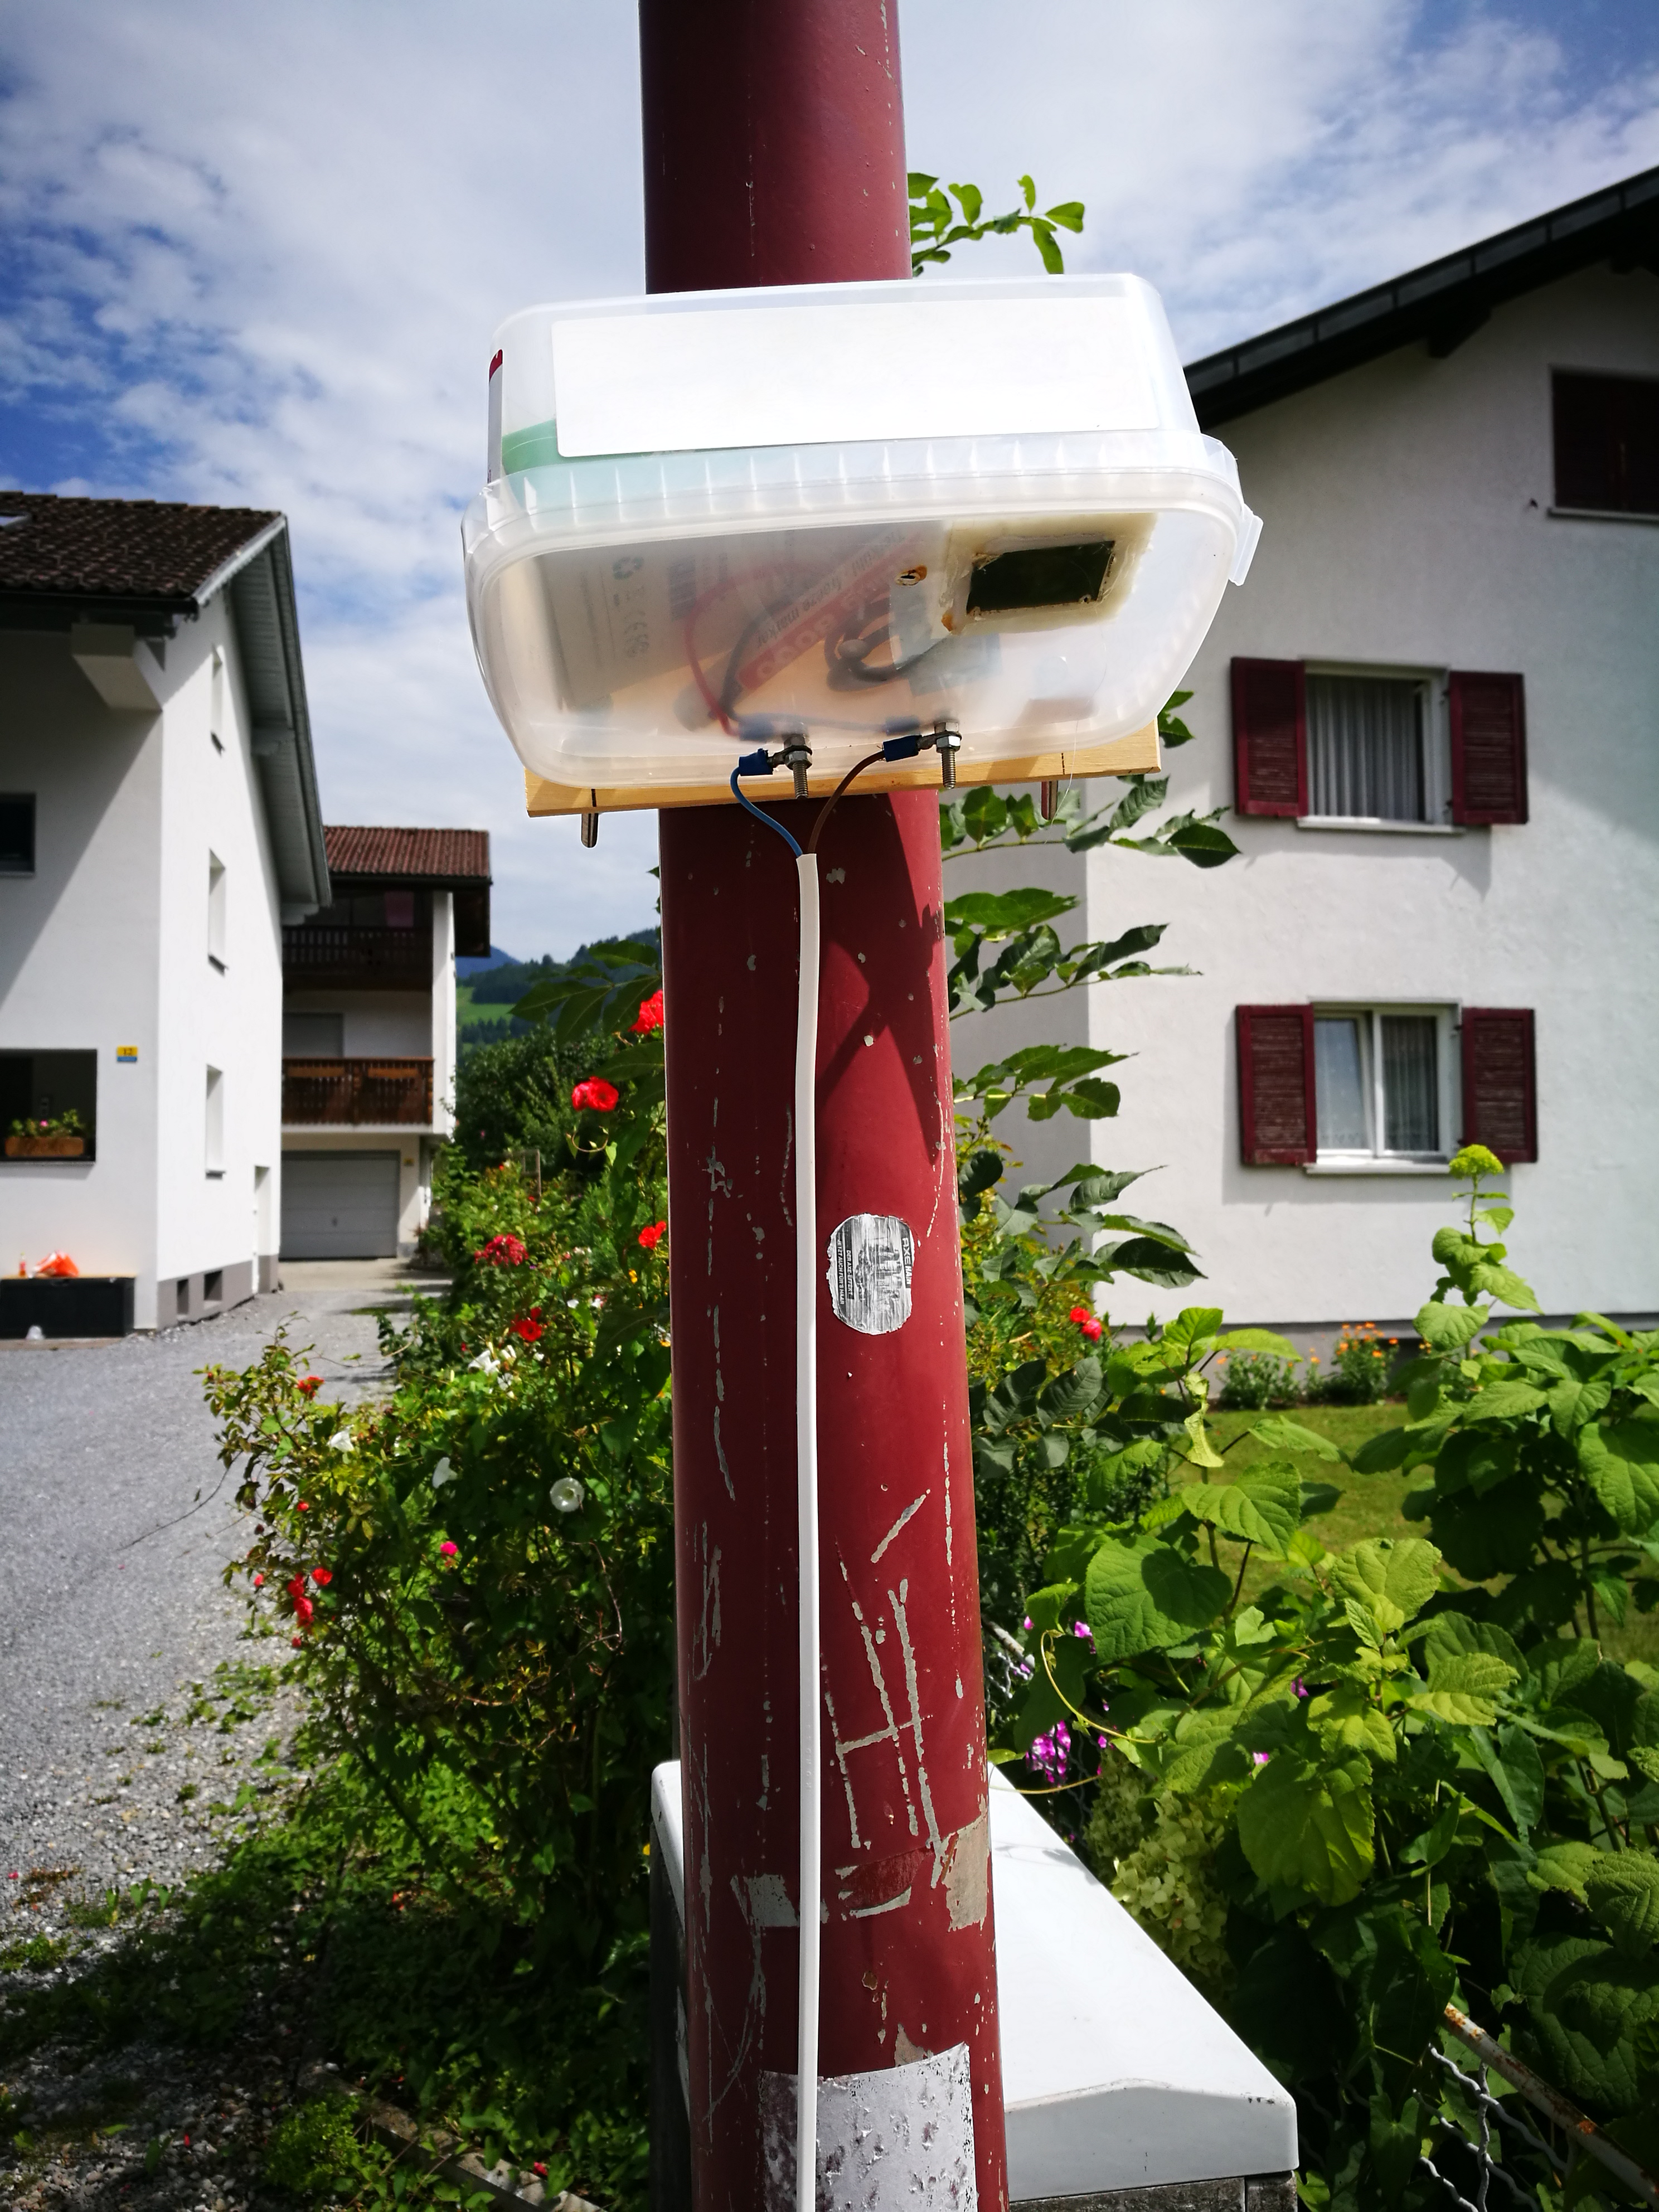
\includegraphics[height=0.6\textwidth]{Hardware/GesamtsystemH.jpg} 
  \caption{Einsatzfähiges Gesamtsystem}
  \label{bGesamtsystemH}
\end{figure}